\section{A potential mechanism: peer interactions}\label{sec:new_theory_peer_effects}


In this section I propose a conceptual framework to interpret the empirical findings. I follow the approach adopted in \cite*{blume2015linear} of micro-founding observed spillover effects through a model of behavior.\par 

In the model, students are heterogeneous with respect to a trait that affects how easy or difficult it is to exert study effort; utility-maximizing effort decisions depend on this trait, which I refer to as effort-cost type.\footnote{Unlike \cite*{blume2015linear}, who assume that students choose achievement directly, I assume that students choose effort, and that effort affects achievement monotonically like in \cite{fruehwirth2013identifying}. This assumption allows me to derive model implications in terms of the observed achievement outcomes. Several studies show empirically that effort increases achievement (\cite{stinebrickner2004time,stinebrickner2008causal,de2010must}), providing strong empirical support to this model's assumption. Good measures of effort are typically unavailable in large scale administrative datasets like the ones used in this study, as they require costly data collections to obtain detailed time diaries; researchers have been able to collect them from smaller samples (see e.g. \cite*{conley2024social}).\label{fn:chooseachievement}} In line with the literature on the technology of skill formation, which views knowledge acquisition as a cumulative process where current investments depend on a lagged stock of skills and lagged inputs (e.g., \cite{todd2003specification,cunha2008formulating,cunha2010estimating}), the model assumes that the effort-cost type varies across students depending on their prior test scores and socioeconomic characteristics (proxying lagged inputs).\footnote{The dependence of current investments on past investments can be micro-founded in different ways. In the studies quoted in the text, it is through the impact of past investments on the current period's initial skills stock, which is complementary with current investments in the skill production technology. Recently, \cite*{caucutt2025child} developed a dynamic life-cycle model of parental investments into child skills in which investments depend on past investments not through technological complementarity, but indirectly through the marginal utility of consumption. In contrast to the literature on the technology of skill formation, my study does not aim to estimate the parameters of the achievement production function; its focus is instead on comparative statics from changing the distribution of peers' effort-cost types. In my model, letting students differ in the cost or productivity of effort would yield the same testable implications.  } Additionally, motivated by the evidence that home damages from the earthquake increased students' perceived cost of study effort (Table \ref{tab:medeffectallni}), I assume that damages affect the effort-cost type as well.\par 


Building on this framework for the student's problem, I present a new theory of peer influence in which exogenous changes to peers’ effort‐cost types affect a student’s own outcomes through a competition motive. When students care about relative performance, changes in peers' effort-cost types change the competition students face, affecting their effort choices and achievement. Empirically, this manifests as a peer effect: exogenous variation in the determinants of peers' effort-cost types, holding fixed a student's own type, causally affects a student's own achievement. In this study, the exogenous variation stems from earthquake shocks. The model's insights, however, are independent of the source of variation in peers' effort-cost types. In particular, whenever prior test scores determine students' effort choices, the model implies that exogenous changes to peers' prior test scores can generate spillover effects if students have rank concerns. The model, therefore, offers a new framework to interpret ability peer effects, a major focus of the empirical peer effects literature.\par
I build on the status game model developed by \cite{hopkins2004running}, where individuals choosing costly consumption care about consumption both in absolute and relative terms, and adapt it to the classroom setting, where students choosing costly effort care about achievement both in absolute and relative terms. While \cite{hopkins2004running} study how exogenous changes in the within-group income distribution affect the equilibrium distribution of consumption, I study how exogenous changes in the within-group distribution of effort-cost types affect the equilibrium distribution of achievement. Additionally, I adapt the model to the earthquake context by incorporating into the achievement technology schools' mitigating responses to the severity of disruptions, and by allowing damage to a student's home to act as an additive shock to the student's effort-cost type. This feature implies that classrooms with different damage distributions, {\itshape ceteris paribus}, also have different distributions of effort-cost types, triggering equilibrium responses through the competition motive.\par 



 I show that the theory can explain the full set of empirical findings, including those that school-level factors alone cannot explain, in a simple and intuitive way.\par 


   
\subsection{A theory of peer influence }\label{sec:model1}

Within a reference group $l$ there is a continuum of students, each indexed by $i$. Students are heterogeneous in terms of effort-cost type $c_i$, which is distributed in the reference group according to a twice continuously differentiable cumulative distribution function (c.d.f.) $G_l(\cdot)$ on $[\underline{c}_l,\bar{c}_l]$, with $\underline{c}_l\geq 0$. The reference group is where interpersonal interactions occur, such as the classroom.\par 



Students choose how much costly effort $e_i$ to exert, and effort increases GPA $y_i$. Utility is increasing in own GPA and in the GPA rank in the reference group. While the empirical analyses used both GPA and a standardized test score as outcome measures, the theory focuses on GPA as its rank is in principle observable by peers. Students with a higher effort-cost type $c_i$ incur a larger cost of exerting study effort for each effort level. Cost type $c_i$ captures all student characteristics, environmental, psychological and socioeconomic, that affect the  ease or difficulty with which a student exerts study effort. For each student $i$, it depends on her baseline test score $a_i$, family characteristics $x_i$, and damages her home incurred from the earthquake $d_i$:\footnote{In this section, I use the notation $x_i$ to denote the vector of student characteristics excluding the fourth-grade standardized test score $a_i$. $x_i$ includes parental education, student's gender, whether the student resides in the school town, region of residence, public school and rural school attendance.}  \par 


\begin{equation}\label{eq:cost_effort}
    c_i=\theta_0+\theta_1 a_i+\theta_2  x_i + \theta_3  d_i.
    \end{equation}


\noindent The cost type $c_i$ is assumed to be decreasing in the baseline test score $a_i$ and increasing in the damages $d_i$, assumptions that are supported in the data  (Table \ref{tab:medeffectallni} and Appendix Figure \ref{fig:eff_cost_simce}). Each student's cost type is private information, but the distribution of cost types in the reference group, $G_l(\cdot)$, is common knowledge. Appendix \ref{sec:model_extension} provides an extension to the model where $c_i$ also depends on an idiosyncratic shock, $\epsilon_i$, that is unobserved by the econometrician. There are no distributional assumptions on $G_l(\cdot)$.\par 

The cost of effort is determined by a strictly increasing and strictly convex function of effort: $q(e_i;c_i)$. Higher cost types $c_i$ incur larger costs for every level of effort $e_i$, i.e., $\frac{\partial q(e_i,c_i)}{\partial c_i}>0$ for all $e_i$. Moreover, at higher cost types the marginal cost of effort is (weakly) higher: $\frac{\partial^2 q(e_i;c_i)}{\partial c_i \partial e_i}\geq 0$. Effort increases GPA according to the production function: 
\vskip-10pt
\begin{equation}\label{eq:y_prod}
    y(e_i)=(a_0+a_1(\mu_{dl}))e_i+u_0+u_1(\mu_{dl}),\quad \mbox{ with } a_0+a_1(\mu_{dl})>0,
\end{equation}



\noindent where  $\mu_{dl}$ is the mean of damages among peers in the reference group.\footnote{Other models of competition between students in the literature make the same assumptions that students are characterized by a type that affects their cost of producing achievement, and that achievement depends only indirectly on their type through the investment choice (\cite{bodoh2017pre,bodoh2018college,cotton2022affirmative}).\label{footnote:R2point4}} The functions $a_1(\mu_{dl}) $ and $u_1(\mu_{dl})$ capture mitigating, compensatory actions taken by schools in response to mean damages in the classroom.\footnote{Alternatively, one could assume that the mitigating action in response to $\mu_{dl}$ directly affects the average cost type in the reference group, thus indirectly affecting $y_i$ in equilibrium. The model's implications would stand. } Mitigation is allowed for but not imposed, as the $u_1$ and $a_1$ functions are allowed to be flat, specifically, it is assumed that $\frac{d a_1(\mu_{dl})}{d \mu_{dl}}\geq 0$ and $\frac{d u_1(\mu_{dl})}{d\mu_{dl}}\geq 0$. Mitigation is allowed to affect either the level of achievement (through $u_1$), or the productivity of effort (through $a_1$), or both; the model is agnostic about which channel drives mitigation efforts. Motivated by the evidence, I do not let mitigation depend on the standard deviation of damages.\par 
The utility function for student $i$ can be decomposed into a utility that depends only on own GPA $y_i$ in absolute terms and on effort cost $q_i=q(e_i,c_i)$, $u_i=V(y_i,q_i)$, and a utility that depends on GPA rank in the classroom. Function $V$ does not have an $i$ subscript because it is the same for all students. The utility from GPA in absolute terms net of effort cost is non-negative, strictly increasing and linear in GPA, strictly decreasing and linear in $q_i$, and it admits an interaction between utility from GPA and from effort cost such that at higher costs, the marginal utility from GPA is (weakly) lower ($V_{12}\leq 0$).\footnote{All results are valid under an alternative set of assumptions for the utility $V$ and cost function $q$. These are: strictly quasi-concave utility from GPA, strictly decreasing and linear utility from cost of effort ($V_2<0,V_{22}=0$) with a linear cost function ($\frac{\partial^2 q}{\partial e_i^2 }=0$) and additive separability between utility from GPA and cost of effort ($V_{12}=0$).} No functional form assumptions are made on $q(\cdot)$ or on the interaction between $y_i$ and $q_i$; the results are valid under a broad class of preferences. For example, students with lower effort-cost type $c_i$ may (or may not) have higher marginal utilities from GPA.\par 
A student's GPA rank in the classroom is given by the within-classroom cumulative distribution function (c.d.f.) of GPA computed at her own GPA, $F_{Yl}(y_i)$, where $l$, like before, refers to the classroom. This is the fraction of students with GPA lower than one's own. Because GPA is an increasing deterministic function of effort, GPA rank equates effort rank: $F_{Yl}(y(e_i))=F_{El}(e_i)$, where $F_{El}(\cdot)$ is the within-classroom c.d.f. of effort. The utility from rank, $S\big(F_{Yl}(y(e_i))\big)$, equals $F_{El}(e_i)+\phi$, with $\phi>0$. Overall utility $U(y_i,q_i)$ is the product of utility from GPA and GPA rank: $V(y_i,q_i)\left(F_{El}(e_i)+\phi\right)$. Each student chooses effort to maximize overall utility.\par 

In a symmetric Nash equilibrium in pure strategies, every student follows the same strategy $e_l(c_i)$ that is such that, given this common strategy, no student $i$ can increase her expected utility by deviating unilaterally. Focusing on such equilibria, and initially assuming that the equilibrium strategy $e_l(c_i)$ is strictly decreasing and differentiable with inverse function $c_l(e_i)$, GPA rank in equilibrium can be rewritten as $1-G_l\big(c_l(e_i)\big)$, and $i$'s utility as $V\big(y(e_i),q(e_i,c_i)\big)\big(1-G_l\big(c_l(e_i)\big)+\phi\big)$.\footnote{Strict monotonicity and differentiability of equilibrium $e_l(c_i)$ are initially assumed, and subsequently proven (see the proof of Proposition \ref{prop1existence} in Appendix \ref{app:theory}). GPA rank can be written as $1-G_l(c_l(e_i))$ in equilibrium because the probability that a student $i$ of type $c_i$ with effort choice $e_i=e_l(c_i)$ chooses a higher effort, obtaining a higher GPA, than another arbitrarily chosen student $j$ in classroom $l$ is $F_{El}(e_i)=Pr\big(e_i>e_l(c_j)\big)=Pr\big(e^{-1}_l(e_i)<c_j\big)=Pr\big(c_l(e_i)<c_j\big)=1-G_l\big(c_l(e_i)\big)$ where $G_l(\cdot)$ is the c.d.f. of $c_i$ in classroom $l$ and $c_l(\cdot)=e^{-1}_l(\cdot)$. The function $c_l$ maps $e_i$ into the type $c_i$ that chooses effort $e_i$ under the equilibrium strategy, it exists by strict monotonicity and, therefore, invertibility of $e_l(\cdot)$. } The first-order condition then is:


\begin{equation}\label{eq:FOC}
\underbrace{V_1 \overbrace{(a_0+a_1(\mu_{dl}))}^{\text{mg. GPA increase}}}_{\text{mg. ut. from increased GPA}}+\underbrace{\frac{V(y_i,q_i)}{1-G_l\big(c_l(e_i)\big)+\phi} 
 \overbrace{g_l\big(c_l(e_i)\big)\big(-c^{\prime}_l(e_i)\big)}^{\text{mg. GPA rank increase}}}_{\text{mg. ut. from increased GPA rank}}=\underbrace{-V_2\frac{\partial q}{\partial e_i}}_{\text{mg. cost}}.
\end{equation}

  The model is an application of the status game in \cite{hopkins2004running}.\footnote{For related games of status models, see also \cite{hoppe2009theory} and \cite{moldovanu2007contests}.} Proposition \ref{prop1existence} in Appendix \ref{app:theory} establishes equilibrium existence and uniqueness and that the equilibrium strategy is indeed strictly decreasing, confirming equation \eqref{eq:FOC} as the appropriate first-order condition.\par 


\subsection{Model predictions and their empirical counterparts}\label{sec:predictions_and_empirical}
\paragraph{Impacts of mean damages on GPA.} The first set of model implications regards the impacts on GPA of increasing mean damages in the classroom while preserving damage dispersion. I consider an identical increase in $d_i$ for all classmates. Consider two classrooms $A$ and $B$ with identical distributions of $a_i$ and $x_i$ (i.e., identical peer compositions), but with different damage distributions $D(\cdot)$: $D_{B}(d)=D_{A}(d-k)$ $\forall d$, where $k$ is a positive constant. That is, the damage distribution in classroom $B$ is shifted to the right by $k$. \par 


\begin{proposition}\label{prop2}
Let $E_A[\cdot]$ and $E_B[\cdot]$ denote classroom-specific expectations. 
Assume that equilibrium effort schedules in classrooms $A$ and $B$ do not cross after the uniform shift in cost types. 
At the Nash equilibrium in each classroom $l=A,B$:

\begin{enumerate}[label=(\roman*),itemsep=0pt,parsep=0pt,topsep=0pt]

\item 
If $\frac{\partial^2 q}{\partial e_i \partial c_i}=0$ and $\frac{d a_1}{d\mu_{dl}}=0$, 
then the model does not deliver a sharp prediction for the sign of $E_B[y_i]-E_A[y_i]$.


\item 
If $\frac{\partial^2 q}{\partial e_i \partial c_i}=0$ and $\frac{d a_1}{d\mu_{dl}}>0$, 
then $E_B[y_i]>E_A[y_i]$.  


\item 
If $\frac{\partial^2 q}{\partial e_i \partial c_i}>0$ and $\frac{d a_1}{d\mu_{dl}}>0$, 
then $\exists \gamma>0$ such that if $\frac{\partial^2 q}{\partial e_i \partial c_i}\le \gamma$, $E_B[e_i]\ge E_A[e_i]$, so that $E_B[y_i]>E_A[y_i]$. If $\frac{\partial^2 q}{\partial e_i \partial c_i}>\gamma$, then $E_B[e_i]<E_A[e_i]$, and  
$E_B[y_i] \ge E_A[y_i]$ or $E_B[y_i]<E_A[y_i]$ depending on the magnitudes of 
$\frac{d a_1}{d\mu_{dl}}$ and $\frac{d u_1}{d\mu_{dl}}$, i.e.\ on whether school action compensates for the decrease in effort.


\item 
If $\frac{\partial^2 q}{\partial e_i \partial c_i}>0$ and $\frac{d a_1}{d\mu_{dl}}=0$, 
then $E_B[e_i]<E_A[e_i]$, and  
$E_B[y_i] \ge E_A[y_i]$ or $E_B[y_i]<E_A[y_i]$ depending on the magnitude of $\frac{d u_1}{d\mu_{dl}}$, 
i.e.\ on whether additive compensatory action through $u_1$ compensates the decrease in effort.

\end{enumerate}
\end{proposition}
 Proof: see Appendix \ref{app:theory}.\par 

Proposition \ref{prop2} states that the impacts on GPA of increasing mean damages in the classroom through a dispersion-preserving shift in the damage distribution depend on schools' compensatory action.\par 
If schools do not implement multiplicative compensatory action ($\frac{d a_1}{d \mu_{dl}}=0$) and if the marginal effort cost increases with own type, then the effect on GPA will be positive or null if additive compensatory action (over)compensates for the decrease in effort, negative otherwise. If instead the marginal effort cost does not vary with own type, the model is agnostic.\par 
If schools adopt multiplicative compensatory action  ($\frac{d a_1}{d \mu_{dl}}>0$), then the impact on GPA will be positive provided each student's marginal effort cost does not vary with own type. If it does, then the impact on GPA will still be positive provided effort cost increases with own type sufficiently slowly such that effort does not decrease ($0< \frac{\partial^2 q}{\partial e_i \partial c_i}<\gamma$), or provided compensatory action (multiplicative, additive, or both) over-compensates for any decrease in effort, otherwise the impact on GPA will be negative or null (in the case of exact compensation).



This result rationalizes the empirical findings that GPA and test scores increased with mean damage, keeping classroom composition constant, suggesting schools took compensatory actions (Table \ref{tab:effectsts}), and that mean damages had insignificant, potentially negative impacts once the effects of schools' compensatory actions are removed using school-by-cohort fixed effects (first column of Figure \ref{fig:heteffects_bysimce_fe}), although the confidence bands for these estimates are large. The result also rationalizes the evidence that schools reallocated SEP resources towards student support in response to mean damages (Section \ref{sec:resources}).\par 


\paragraph{Impacts of dispersion in damages on GPA.}  The second set of model implications regards the impacts on GPA of increasing damage dispersion in the classroom while keeping mean damages constant. I consider an increase in dispersion in the unimodal likelihood ratio (ULR) sense. Consider two classrooms $A$ and $B$ with identical distributions of $a_i$ and $x_i$ (i.e., identical peer compositions), but with different damage distributions $D(\cdot)$: $D_A \succ_{ULR} D_B$, that is, the ratio of the densities $L(d_i)=\frac{d_A(d_i)}{d_B(d_i)}$ is strictly increasing for $d_i<\tilde{d}$ and strictly decreasing for $d_i>\tilde{d}$ for some $\tilde{d}\in[\underline{d},\bar{d})$ and $\mu_{dA}=\mu_{dA}$. In particular, if $B$ has the same mean but higher variance than $A$, then $D_A \succ_{ULR} D_B$. We restrict attention to changes in the dispersion of $d$ such that the effort-cost-type distributions satisfy the same ULR order, $G_A\succ_{ULR} G_B$, with cutoff point $\tilde{c}\in[\underline{c},\bar{c})$. Figure \ref{fig:sim_viz} visualizes the effort-cost type distributions of two classrooms where the distributions of $a_i$ and $x_i$ are identical (blue density functions in the two top panels), and the damage distribution in classroom B is a mean-preserving spread of that in classroom A. The resulting effort-cost type distribution in classroom B is a mean-preserving spread of that in classroom A (bottom panel).\par


\begin{figure}[h!]
    \centering
    \begin{subfigure}[b]{0.45\textwidth}
        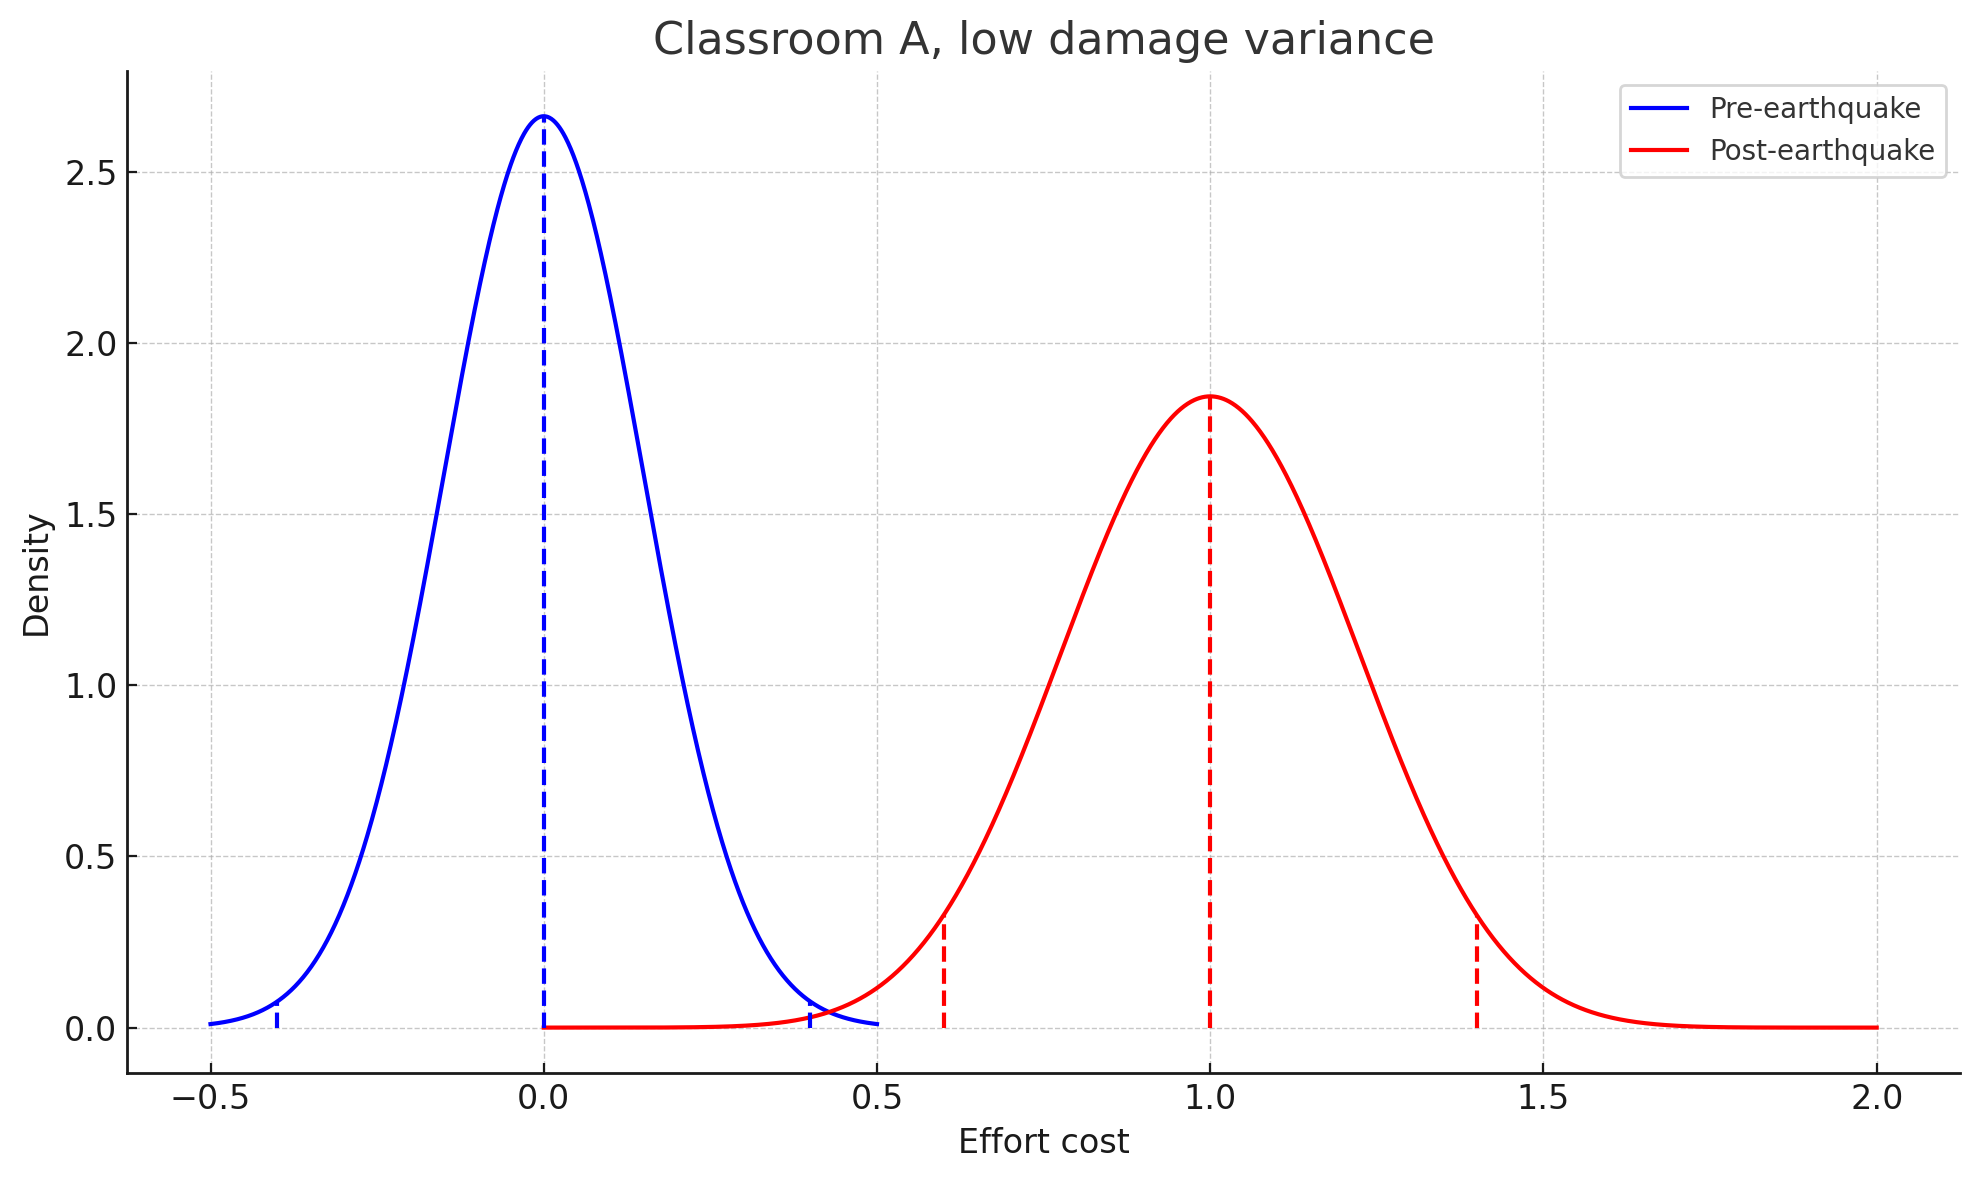
\includegraphics[width=\textwidth]{Paper/classroomA_additive_damage.png}
        \caption{Classroom A, low damage variance}
    \end{subfigure}
    \hfill
    \begin{subfigure}[b]{0.45\textwidth}
        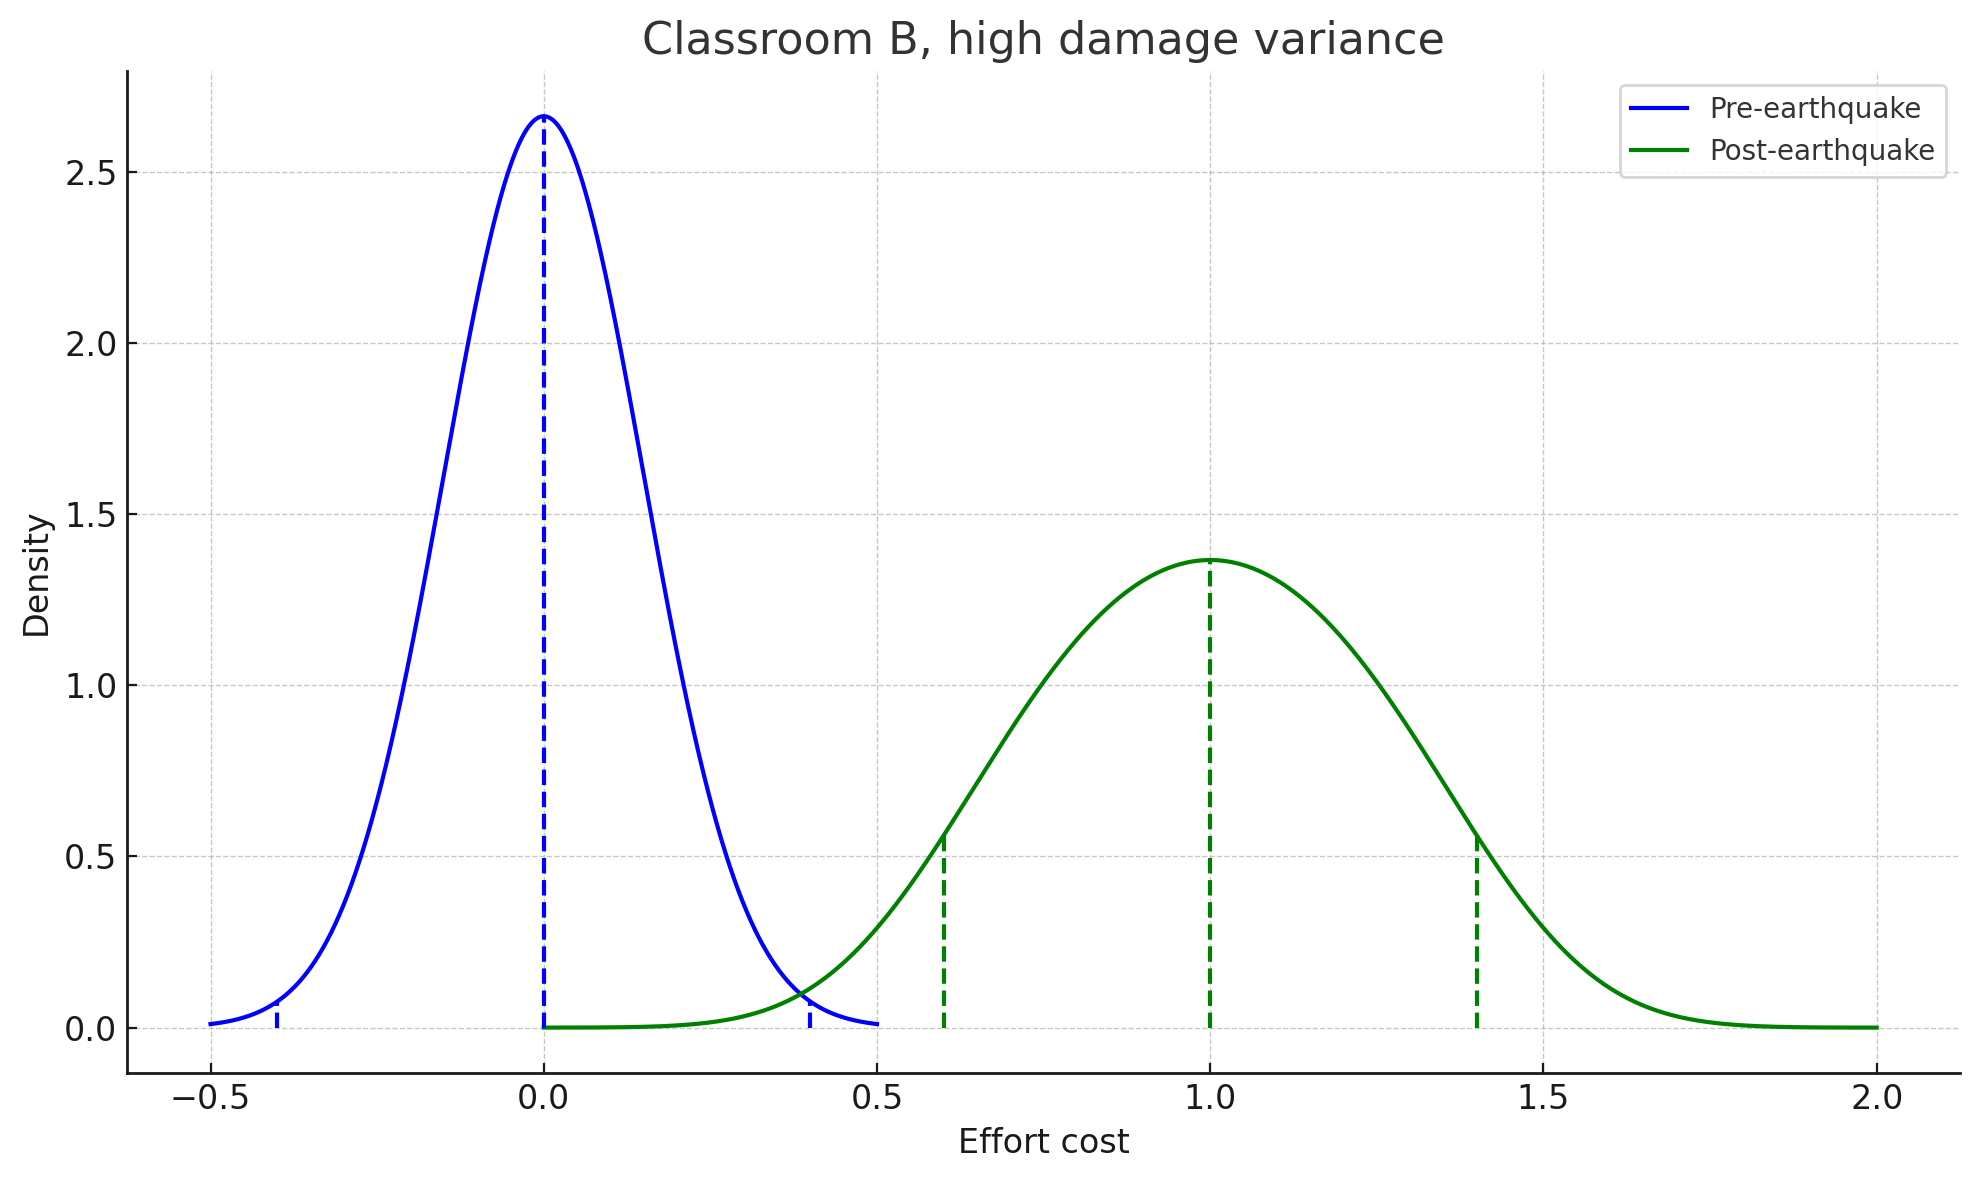
\includegraphics[width=\textwidth]{Paper/classroomB_additive_damage.png}
        \caption{Classroom B, high damage variance}
    \end{subfigure}

    \vspace{1em}
    
    \begin{subfigure}[b]{0.45\textwidth}
        \centering
        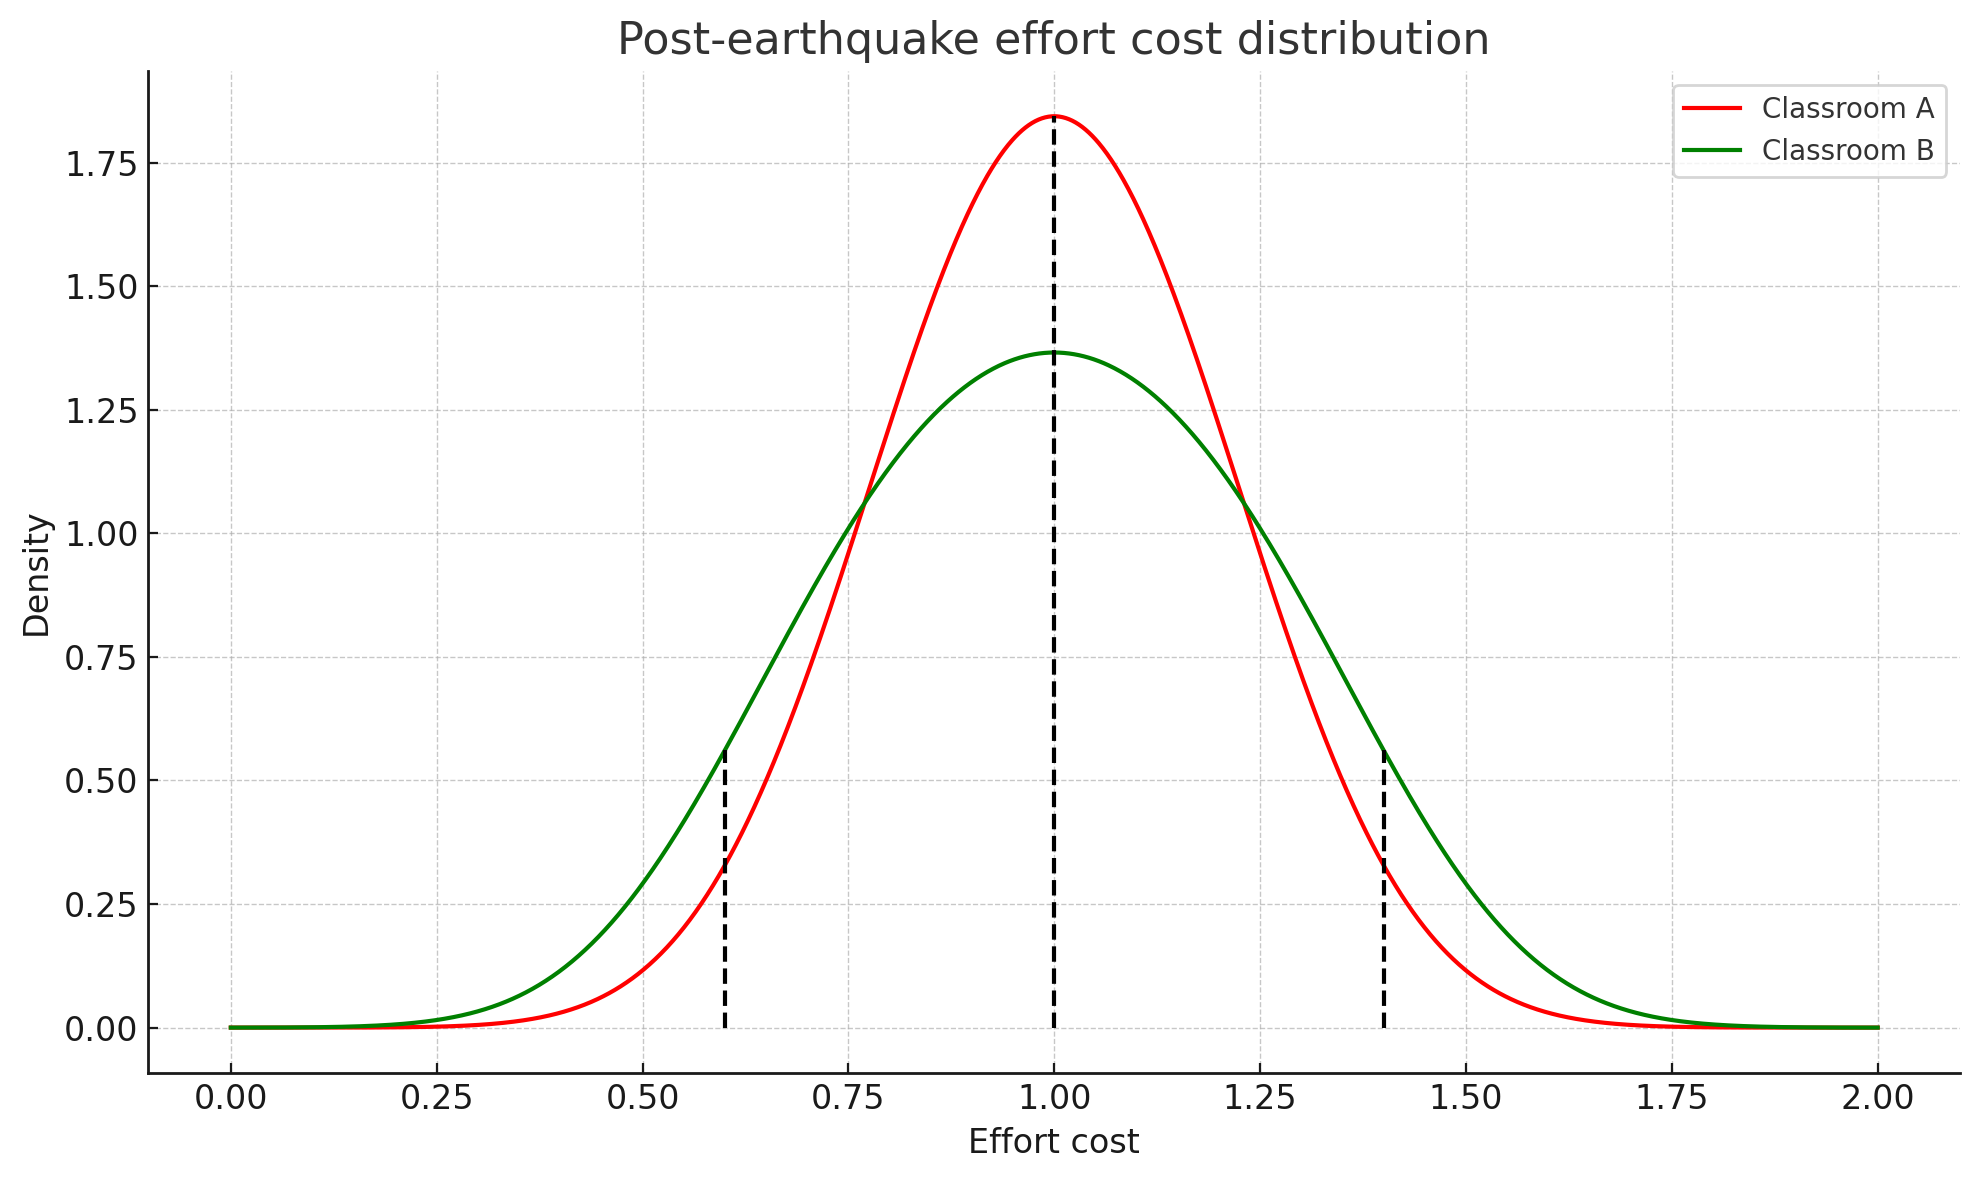
\includegraphics[width=\textwidth]{Paper/classrooms_AB_post_earthquake_additive_damage.png}
        \caption{Classrooms A and B: Post-Earthquake effort-cost type distributions}
    \end{subfigure}

 \caption{Effect of different damage shock distributions on the effort-cost type distributions of two initially identical classrooms. {\itshape Notes:} The pre-earthquake effort-cost type distribution is represented by a normal distribution \(X \sim N(0, 0.15)\), drawn in blue. It captures the portion of effort-cost type influenced only by student baseline test score and individual characteristics. After the earthquake, the damage distribution in classroom A is described by \(D_A \sim N(1, 0.21)\) and in classroom B by \(D_B \sim N(1, 0.38)\). The post-earthquake effort-cost type is the summation of component \(X\) (influenced by student characteristics and lagged test score) and the damage. Specifically, for classroom A it is given by \(X_{\text{post,A}} = X + D_A\) and for classroom B by \(X_{\text{post,B}} = X + D_B\), whose distributions are drawn in red and green.}
    \label{fig:sim_viz}
\end{figure}



\begin{proposition}\label{prop3} \textnormal{(Adapted from Proposition 4 in \cite{hopkins2004running}).} Let \( y_A(c_i) \) and \( y_B(c_i) \) denote the GPA each effort-cost type $c_i$ obtains at the Nash Equilibrium choices of effort in classrooms $A$ and $B$, and let $c^{-}$ and $c^{+}$ denote the extremal points of the ratio $(1-G_A(c_i))/(1-G_B(c_i))$ over the interval $[\underline{c},\bar{c}]$, where $\underline{c}<c^{-}<c^{+}\leq\bar{c}$. Then:
\begin{enumerate}[label=(\roman*),itemsep=0pt,parsep=0pt,topsep=0pt]
\item $y_A(c_i)<y_B(c_i)$ for all $c_i\in [c^{+},\bar{c}]$; i.e., the damage dispersion increase raises the GPA of high-cost-type students.
\item $y_A(c_i)>y_B(c_i)$ for all $c_i\in[\tilde{c},c^{cross})$, where $c^{cross}\in(\tilde{c},c^{+})$ is the point where $y_A$ and $y_B$ cross; i.e., the damage dispersion increase lowers the GPA of medium-cost-type students.  
\item $y_A(c_i)>y_B(c_i)$ for all $c_i\in [\underline{c},\tilde{c})$ or $y_A(c_i)<y_B(c_i)$ for all $c_i\in [\underline{c},c^{cross2})$, where $c^{cross2}\in[\underline{c},c^{-})$ is the point where $y_A$ and $y_B$ cross, i.e., the damage dispersion increase may lower or increase the GPA of low-cost-type students.
\end{enumerate}

\end{proposition}

 Proof: see Appendix \ref{app:theory}.\par 
This proposition states that when students have rank concerns, changing the dispersion of damages and, hence, of effort-cost-types has heterogeneous effects across the cost-type distribution, because it affects differently the incentives to exert effort of different students depending on their position in the distribution. Such heterogeneous effects arise even when the standard deviation of damages does not directly enter the technology of achievement production, such as through an interaction with effort. The intuition is that when students have rank concerns, the cost-type density at one's own type determines how easy it is to improve one's rank. If there are more peers with a similar effort-cost type to one's own, more students can be surpassed for a marginal increase in effort, causing a higher marginal utility of effort. We expect heterogeneous effects because increasing the type dispersion affects the type density differently at different points, increasing it at the tails and lowering it in the middle of the distribution, as can be seen in Panel (c) of Figure \ref{fig:sim_viz}.\par
High- and low-cost-type students face an incentive to increase effort, and medium-cost-type students to decrease it, because of how the type density changes at their type level when the type dispersion increases. The model predicts that high- and middle-cost-type students behave according to these incentives. Low-cost-type students, however, also face the opposite incentive to decrease effort due to the lower competition from above (from the middle-cost types), which allows them to save on effort cost while not sacrificing rank. The model is agnostic as to which incentive prevails for low-cost-type students.\par 

\begin{lemma}\label{lemma}
Proposition \ref{prop3} can be recast in terms lagged test score instead of effort-cost type. Given equation \eqref{eq:cost_effort}, if $x_i=x_j$ and $d_i=d_j$ for $i\neq j$, then $c_i>c_j\iff a_i<a_j$.   
\end{lemma}




Proposition \ref{prop3} and Lemma \ref{lemma} rationalize the empirical findings that, keeping a student's own characteristics and damage constant, achievement and GPA decreased for high-baseline-test-score students and increased for low-baseline-test-score students as an effect of increased damage dispersion, holding classroom composition constant (Table \ref{tab:heteffectsts} and Figures \ref{fig:me_nofe} and \ref{fig:heteffects_bysimce_fe}).\footnote{Appendix \ref{sec:shocks_effort} provides the regression specification that holds classroom composition constant and that is such that, under the specification for the effort-cost type in equation \eqref{eq:cost_effort}, shifts in the classroom mean (Proposition \ref{prop2}) or standard deviation (Proposition \ref{prop3}) of damages translate into shifts in the classroom mean or standard deviation of effort-cost types. Appendix \ref{sec:model_extension} shows under what assumptions this specification remains valid when the effort-cost type is allowed to depend on an unobserved idiosyncratic shock.}  \par 
 
\paragraph{Impacts on GPA rank.} Changing the classroom distribution of damages changes that of effort-cost types. What are the implications on GPA rank, when students draw utility from rank? Consider two classrooms $A$ and $B$ with identical distributions of $a_i$ and $x_i$ (i.e., identical peer compositions), but different distributions of damages $d_i$. The resulting cumulative distribution functions of effort-cost types, $G_A$ and $G_B$, are assumed to be twice continuously differentiable, so that Proposition \ref{prop1existence} applies.\par 

\begin{proposition}\label{prop4} Let $y_A(c_i)$ and $y_B(c_i)$ denote the GPA each cost type $c_i$ obtains at the Nash Equilibrium choices of effort in classrooms A and B. Let $F_Y^J(\cdot)$ denote the c.d.f. of GPA in classroom $J\in\{A,B\}$, and $F_{T}(\cdot)$ the c.d.f. of baseline test score $a_i$ in classrooms A and B. Then, $F_Y^J(y_i)|_{x,d}=F_T(a_i)|_{x,d}$ $\forall J, a_i$; i.e., at given values of $x_i$ and $d_i$, rank in GPA conditional on the baseline test score is identical across classrooms, for all baseline test scores.

\end{proposition}
 Proof: see Appendix \ref{app:theory}.\par 

Proposition \ref{prop4} states that, keeping fixed characteristics $x_i$ and damage $d_i$, the mapping between a student's baseline test score and her classroom GPA rank stays constant, regardless of the distribution of damages in the classroom. As we change the damage distribution, students with higher baseline test scores --- {\itshape ceteris paribus} --- remain those with higher GPA rank. \par 
This result rationalizes the empirical finding that changing the mean or the standard deviation of damages in the classroom, controlling for students' characteristics and individual damages, does not have statistically detectable effects on GPA rank at any point of the baseline test scores distribution (Figures \ref{fig:me_grank_bysimce_nofe} and \ref{fig:heteffectsGPArankmean}), even when it affects GPA.\par 

\subsection{Summary of results}
 Schools' mitigating actions in the achievement production function rationalize the positive impacts of mean damages on achievement and are consistent with observed school resource reallocations. To account for the remaining empirical patterns, I model social interactions among students. The model of rank concerns not only intuitively explains the lack of shifts to GPA rank despite shifts to GPA, but also rationalizes the heterogeneous effects of damage dispersion among students with different initial performance. These seemingly unrelated findings can be explained through one simple modification to standard models of social interactions in schools: the introduction of a desire to compete for grades. The theory provides insights into the nature of social interactions in schools that apply beyond the quasi-experimental empirical context used to formulate it. \par 
